\usepackage{xcolor}
\usepackage[margin=1in]{geometry}
\begin{document}
\lstset{
    frame=single,
    basicstyle=\ttfamily,
    keywordstyle=\color[rgb]{0.13,0.29,0.53}\bfseries,
    stringstyle=\color[rgb]{0.31,0.60,0.02},
    commentstyle=\color[rgb]{0.56,0.35,0.01}\itshape,
    numberstyle=\footnotesize,
    stepnumber=1,
    numbersep=5pt,
    showspaces=false,
    showstringspaces=false,
    showtabs=false,
    tabsize=2,
    captionpos=b,
    breaklines=true,
    breakatwhitespace=true,
    breakautoindent=true,
    escapeinside={\%*}{*)},
    linewidth=\textwidth,
    basewidth=0.5em,
}
\section{EECS 4313: Assignment 2}\label{eecs-4313-assignment-2}

Monday, 29 February 16

\subsection{Team Members}\label{team-members}

\begin{lstlisting}
- Drew Noel (212513784)
- Skyler Layne (212166906)
- Siraj Rauff (212592192)
\end{lstlisting}

\newpage

\section{Method Test \#1:}\label{method-test-1}

The method under investigation, \lstinline!calculateRepeatNumber! exists
within \lstinline!Repeat.java! in the \lstinline!net.sf.borg.model!
package, and has the following signature including java doc:

\begin{lstlisting}[language=Java]
/**
 * Calculate the number of a repeat given the date and the appointment
 *
 * @param current
 *            the date
 * @param appt
 *            the appointment
 *
 * @return the number of the repeat (starting with 1)
 */
final static public int calculateRepeatNumber(Calendar current, Appointment appt)
\end{lstlisting}

The method calculates the instance number of the specified repeating
event on a particular date. This means that a repeating event will have
its instances numerated, and the instance number on the given date will
be rturned.

\begin{itemize}
\tightlist
\item
  The first parameter \textbf{current}, of type \lstinline!Calendar!,
  contains the date for which the instance number is to be determined.
\item
  The second parameter \textbf{appt}, of type \lstinline!Appointment!,
  contains the event specifics including the start date and repeat
  frequency.
\end{itemize}

If a date is given such that it does not exist in the repetitions
(\emph{i.e.} a weekend for a event repeating on weekdays, or a date
before the start date), the value \lstinline!0! is returned.

\subsection{Boundary Value Testing}\label{boundary-value-testing}

Having observed the behavior and documentation of the function, it was
determined that the distances between the start date of the
\lstinline!Appointment! and the \lstinline!Calendar! date should be
pushed to extreme Integer values. This was chosen after inspection of
the code revealed that the repetition was calculated using a loop
tracking an integer value, without proper checking for overflow.

Note that the \lstinline!Appointment! parameter was not Boundary tested
as its use in this function was limited to its start date and repeating
frequency. The lowest frequency value in BORGCalendar was
\lstinline!DAILY!, therefore we could not test for multiple instances
for a given date, and testing for different values would fall within the
scope of testing \lstinline!Calendar!. Testing for extreme values of a
start date would not prove to be useful as we would be testing Java's
\lstinline!DATE! class, and not the method at hand.

Given a specific \lstinline!Appointment!, the following cases were then
chosen for the \lstinline!Calendar!: - The same day - The next day - The
previous day - Integer.MAX\_VALUE - 1 days in the future -
Integer.MAX\_VALUE days in the future - Integer.MAX\_VALUE + 1 days in
the future - Integer.MIN\_VALUE + 1 days in the past -
Integer.MIN\_VALUE days in the past - Integer.MIN\_VALUE - 1 days in the
past

\subsection{Special Value Testing}\label{special-value-testing}

Due to the nature of the \lstinline!Appointment! parameter, in
particular its use for start date and repeating frequency, two special
cases were considered: - Appointment without a start date - Appointment
with no frequency

These were tested to ensure the method was robust, as this custom class
does not ensure that these two fields are set upon creation or
modificaiton.

\section{Method Test \#2:}\label{method-test-2}

The method under test belongs to the \lstinline!EncryptionHelper! class,
located in the package \lstinline!net.sf.borg.common!. The method has
the following signature, including java doc:

\begin{lstlisting}[language=Java]
/**
* encrypt a String using a key from the key store
*
* @param clearText
*            - the string to encrypt
* @param keyAlias
*            - the encryption key alias
* @return the encrypted string
* @throws Exception
*/
public String encrypt(String clearText, String keyAlias);
\end{lstlisting}

This method accepts two arguments: a string which should be encrypted,
and a string which informs the method which key from the
\lstinline!Keystore! to use. The \lstinline!Keystore! is created through
static methods in the class ahead of time. This method throws an
\lstinline!Exception! if there is any type of exception thrown during
its execution.

The technique selected to test this method is the Boundary-Value Test
strategy. Through examining the source code, it is clear that
\lstinline!keyAlias! is only manipulated by core Java methods and
classes, and so testing values of \lstinline!keyAlias! was given a lower
priority. The argument \lstinline!clearText! accepts any
\lstinline!String! as input. By treating the length of the string as the
component to test, the following value breakdown was created:

\begin{itemize}
\tightlist
\item
  A string with zero length
\item
  A string with length of one
\item
  A string with a nominal length
\item
  A string which is exceptionally large
\item
  A string comprised of binary data
\end{itemize}

It is not possible to perform a Strong Boundary-Value Test because a
String cannot have length that is negative, and String has no practical
upper limit. Note that it would be possible to design a test which
forcibly exhausts the memory of the JVM by creating an enormous string
as input. However this would be a failure point on the JVM, which the
application is not expected to be able to handle.

The final test value was created after inspecting the source code. In
the method, there is a call to the \lstinline!String! method
\lstinline!getBytes()!. This method uses the default encoding, which may
or may not fundamentally change the data it receives.

By changing the value of \lstinline!keyAlias! to be either a valid key
or an invalid key (similar to a boolean), a second breakdown was
created:

\begin{itemize}
\tightlist
\item
  A string which describes a valid key
\item
  A string which does not describe a valid key
\end{itemize}

The tests were written to attempt every possible combination of these
test values, creating a Worst-Case Boundary-Value Test suite.
Examination of the source code indicated that the result of an invalid
key description will always be a thrown \lstinline!Exception!.
Specifically the type of the exception will be an
\lstinline!InvalidKeyException!. There were several other types of
exceptions that this method might throw, but since the signature
indicates it may throw any \lstinline!Exception!, this was not tested.

All the tests described above passed when execute. It is worthwhile to
observe that this method, like most methods in the
\lstinline!net.sf.borg.common! package, gives no information about the
exception types that it might throw. This significantly increases the
amount of code that the client classes will require in order to properly
determine why an exception was thrown at all.

\section{Method Test \#3:}\label{method-test-3}

The method under test has the following signature, including java doc:

\begin{lstlisting}[language=Java]
/**
 * Gets the "N" multiplier value from the encoded appointment string
 *
 * @param f
 *            the encoded appointment string
 *
 * @return the "N" multiplier value
 */
static public int getNValue(String f);
\end{lstlisting}

Using the testing techniques which we have discussed in class we have
devised the following strategy for testing the above stubbed method.
Upon inspection, the method under test takes as an argument a
\lstinline!String!. This was troublesome at first however, looking
further into this we were able to deduce what, in this case, a valid
\lstinline!String! is. In this context a valid input string is one which
contains some word, \emph{Constant}, and a comma separated integer,
\emph{Number} such that it has the form \lstinline!"Constant,Number"!.
In the context of testing we can break this up into essentially \emph{2}
inputs, the Constant and the Number. This is important to note from the
start as we use this context through the entire test.

\subsection{Boundary Value Testing}\label{boundary-value-testing-1}

As the input is a \lstinline!String! and the output is an
\lstinline!int!, we can carefully consider the edge cases given that the
input is of the form \lstinline!Constant + "," + Number! (See Appendix A
for the JUnit test cases for this strategy):

\textbf{Constant}:\\
- The empty \lstinline!String!.\\
- A very long \lstinline!String!.\\
- A desirable \lstinline!String!.\\
- Without a comma separator.

\textbf{Number}:\\
- The empty \lstinline!String!.\\
- A non-numeric \lstinline!String!.\\
- A very large negative \lstinline!int! and \lstinline!float!.\\
- Zero.\\
- A very large positive \lstinline!int! and \lstinline!float!.

\subsection{Equivalence Class Testing}\label{equivalence-class-testing}

Using the following strategy we attempt to cover some of the missing
gaps, and remove some of the redundancy from the \emph{Boundary Value
Tests}. The following diagrams present this testing strategy, each of
the possible Number inputs are on the Y axis, while each of the possible
Constant inputs are on the X axis. Each of the filled in boxes presents
valid input, while the X represents a corresponding test case (See
Appendix A for the JUnit test cases for this strategy).

\begin{figure}[htbp]
\centering
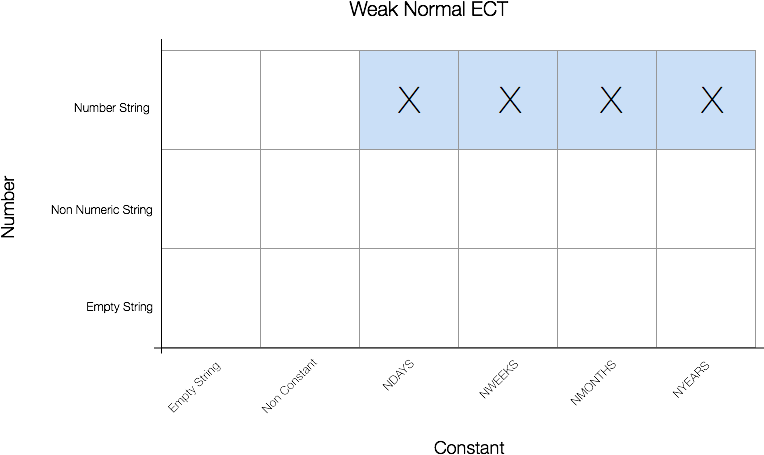
\includegraphics{../assets/weak-normal.png}
\caption{Weak Normal Test Cases}
\end{figure}

\begin{figure}[htbp]
\centering
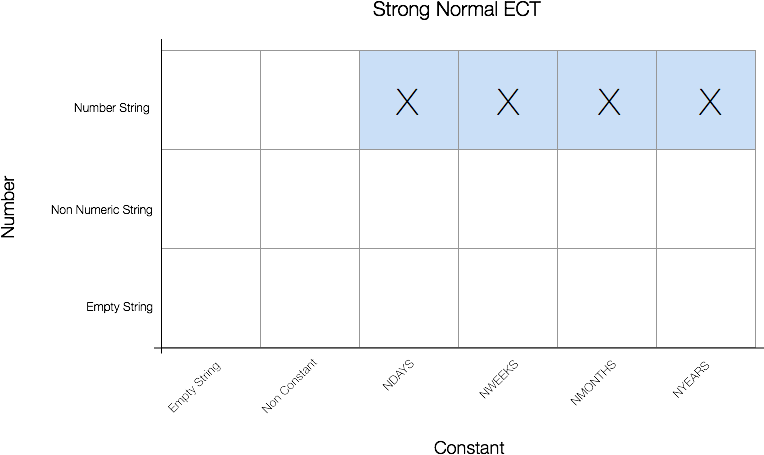
\includegraphics{../assets/strong-normal.png}
\caption{Strong Normal Test Cases}
\end{figure}

\begin{figure}[htbp]
\centering
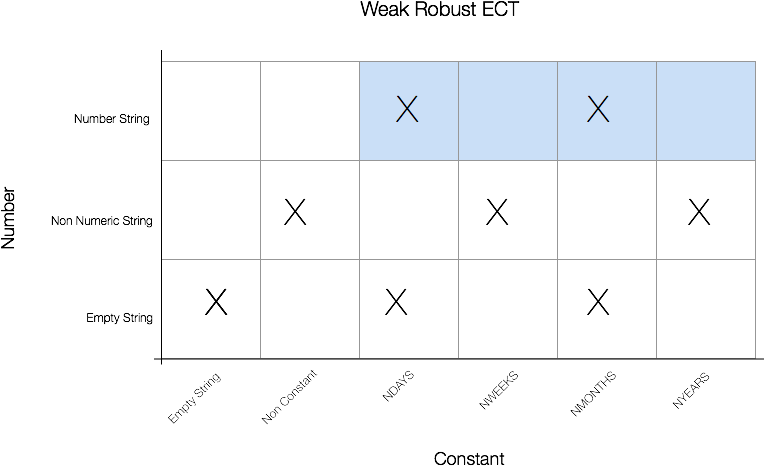
\includegraphics{../assets/weak-robust.png}
\caption{Weak Robust Test Cases}
\end{figure}

\begin{figure}[htbp]
\centering
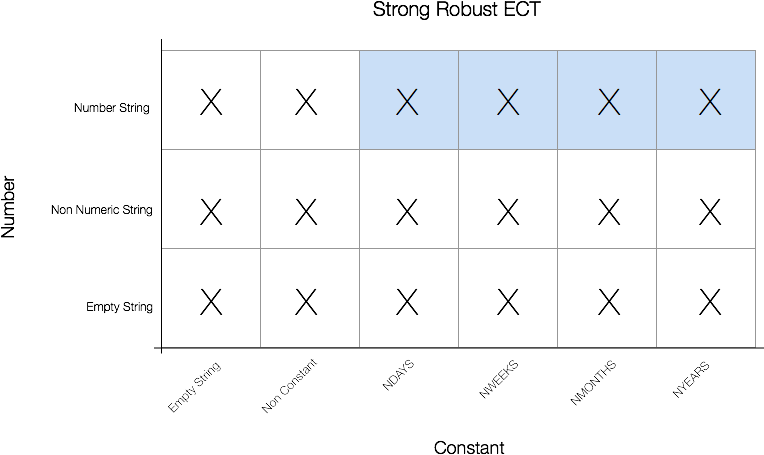
\includegraphics{../assets/strong-robust.png}
\caption{Strong Robust Test Cases}
\end{figure}

\newpage

\subsection{Decision Table Testing}\label{decision-table-testing}

In the following decision table we show the desired behaviour of the
system; under the condition what the desired action should be (See
Appendix A for the JUnit test cases for this strategy).

\begin{figure}[htbp]
\centering
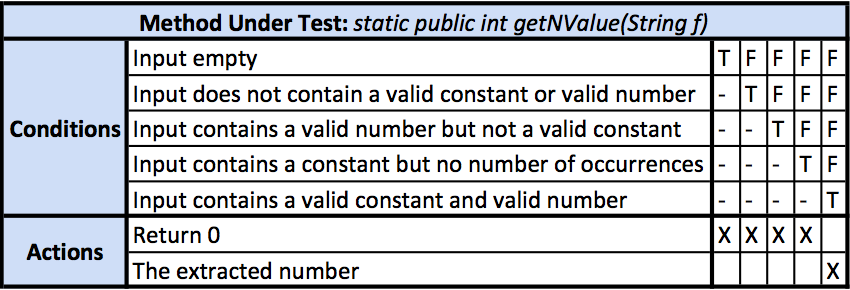
\includegraphics{../assets/decision-table.png}
\caption{Decision Table}
\end{figure}

\newpage

\section{Appendix A}\label{appendix-a}

\subsection{Bug Report \#1}\label{bug-report-1}

\textbf{Title}: Integer Overflow in \lstinline!calculateRepeatNumber!.\\
\textbf{Reported by}: Siraj Rauff.\\
\textbf{Date Reported}: February 28, 2016.\\
\textbf{Program name}: BORG Calendar.\\
\textbf{Configuration}: OS X 10.11.3, Java version 1.8.0\_71, Runtime
build 1.8.0\_71-b15.\\
\textbf{Report type}: Bug.\\
\textbf{Reproducibility}: Yes -- consistently.\\
\textbf{Priority}: Medium.\\
\textbf{Problem Summary}:\\
\lstinline!calculateRepeatNumber! in \lstinline!Repeat.java! does not
account for integer overflow in its calculation.\\
\textbf{Problem Description}:\\
\lstinline!calculateRepeatNumber! utilizes a for loop, keeping track of
the number of occurrences of the repeating event using an integer
variable. (\lstinline!Repeat.java!, {[}446,0{]})

\begin{lstlisting}[language=Java]
for (int i = 1;; i++) { ... }
\end{lstlisting}

This section of the method does not, however, check for integer
overflow. This means that any event that occurs more than
\lstinline!Integer.MAX_VALUE! times, the method will simply wrap around
to \lstinline!Integer.MIN_VALUE! and continue counting. Depending on the
implementation of infinitely repeating events, a event could quite
reasonably have more than \lstinline!Integer.MAX_VALUE! instances.

This can be reproduced with the following:

\begin{lstlisting}[language=Java]
Calendar testCal = new GregorianCalendar(0,0,1,0,0);
Appointment testAppt = new Appointment();
testAppt.setFrequency("DAILY");
testAppt.setDate(testCal.getTime());

testCal.add(Calendar.DAY_OF_MONTH, Integer.MAX_VALUE);
testCal.add(Calendar.DAY_OF_MONTH, 1);
assertEquals(greaterThan(Integer.MAX_VALUE), Repeat.calculateRepeatNumber(testCal, testAppt));
\end{lstlisting}

\textbf{New or old bug}: old.

\subsection{Bug Report \#2}\label{bug-report-2}

\textbf{Title}: Unchecked \lstinline!NullPointerException! in
\lstinline!calculateRepeatNumber!.\\
\textbf{Reported by}: Siraj Rauff.\\
\textbf{Date Reported}: February 28, 2016.\\
\textbf{Program name}: BORG Calendar.\\
\textbf{Configuration}: OS X 10.11.3, Java version 1.8.0\_71, Runtime
build 1.8.0\_71-b15.\\
\textbf{Report type}: Bug.\\
\textbf{Reproducibility}: Yes -- consistently.\\
\textbf{Priority}: Low.\\
\textbf{Problem Summary}:\\
\lstinline!calculateRepeatNumber! in \lstinline!Repeat.java! does not
check if the \lstinline!Appointment! contains a valid start date before
using it.\\
\textbf{Problem Description}:\\
\lstinline!calculateRepeatNumber! utilizes an \lstinline!Appointment!
parameter to get the start date and repeat frequency of an event. It
does not, however, check if either of these exist. A \lstinline!null!
frequency is correctly handled in the creation of a repeating event,
however a \lstinline!null! start date will cause a
\lstinline!NullPointerException!.

This can be reproduced with the following:

\begin{lstlisting}[language=Java]
Calendar testCal = new GregorianCalendar(0,0,1,0,0);
Appointment testAppt = new Appointment();

assertEquals(0, Repeat.calculateRepeatNumber(testCal, testAppt));
\end{lstlisting}

\textbf{New or old bug}: old.

\subsection{Bug Report \#3}\label{bug-report-3}

\textbf{Title}: Unchecked NumberFormatException.\\
\textbf{Reported by}: Skyler Layne.\\
\textbf{Date Reported}: February 28, 2016.\\
\textbf{Program name}: BORG Calendar.\\
\textbf{Configuration}: OS X 10.11.3, Java version 1.8.0\_60, Runtime
1.8.0\_60-b27.\\
\textbf{Report type}: Bug.\\
\textbf{Reproducibility}: Yes -- consistently.\\
\textbf{Priority}: Low.\\
\textbf{Problem Summary}:

Unit testing surfaced an uncaught error in String to Integer conversion.

When setting a repeat event, if the String code passed in takes space,
or if it is not an integer, then an uncaught/unhandled error occurs
\lstinline!NumberFormatException! error occurs. Example inputs:

\begin{lstlisting}[language=Java]
Repeat.getNValue("nweeks, ");
Repeat.getNValue("nweeks, 14");
Repeat.getNValue("nweeks, FOO");
Repeat.getNValue("nweeks,FOO");
\end{lstlisting}

\textbf{New or old bug}: New.

\newpage

\section{Appendix B}\label{appendix-b}

\subsection{Method \#1}\label{method-1}

\subsubsection{Boundary Value Tests}\label{boundary-value-tests}

\begin{lstlisting}[language=Java]
/*
 * Testing Boundry Values of Calculate Repeat Number
 */
@Test
public void testCalculateRepeatNumberBVT() {

  /*
   * Boundary Values for Calendar:
   * 1. The same day
   * 2. The next day
   * 3. The previous day
   * 4. Integer.MAX_VALUE - 1 days in the future
   * 5. Integer.MAX_VALUE days in the future
   * 6. Integer.MAX_VALUE + 1 days in the future
   * 7. Integer.MIN_VALUE + 1 days in the past
   * 8. Integer.MIN_VALUE days in the past
   * 9. Integer.MIN_VALUE - 1 days in the past
   */

  Calendar prevDay = new GregorianCalendar(0,0,1,0,0);
  Calendar sameDay = new GregorianCalendar(0,0,2,0,0);
  Calendar nextDay = new GregorianCalendar(0,0,3,0,0);
  Appointment sampleAppt = new Appointment();
  sampleAppt.setFrequency("DAILY");

  // 1. The same day
  sampleAppt.setDate(sameDay.getTime());
  assertEquals(1, Repeat.calculateRepeatNumber(sameDay, sampleAppt));

  // 2. The next day
  assertEquals(2, Repeat.calculateRepeatNumber(nextDay, sampleAppt));

  // 3. The previous day
  assertEquals(0, Repeat.calculateRepeatNumber(prevDay, sampleAppt));

  // 4. Integer.MAX_VALUE - 1 days in the future
  Calendar overMaxDays = sameDay;
  overMaxDays.add(Calendar.DAY_OF_MONTH, Integer.MAX_VALUE - 1);
  assertEquals(Integer.MAX_VALUE, Repeat.calculateRepeatNumber(overMaxDays, sampleAppt));

  // 5. Integer.MAX_VALUE days in the future
  overMaxDays.add(Calendar.DAY_OF_MONTH, 1);
  assertEquals(greaterThan(Integer.MAX_VALUE), Repeat.calculateRepeatNumber(overMaxDays, sampleAppt));

  // 6. Integer.MAX_VALUE days in the future
  overMaxDays.add(Calendar.DAY_OF_MONTH, 1);
  assertEquals(greaterThan(Integer.MAX_VALUE), Repeat.calculateRepeatNumber(overMaxDays, sampleAppt));

  // 7. Integer.MIN_VALUE + 1 days in the past
  Calendar underMaxDays = sameDay;
  underMaxDays.add(Calendar.DAY_OF_MONTH, Integer.MIN_VALUE + 1);
  assertEquals(0, Repeat.calculateRepeatNumber(underMaxDays, sampleAppt));

  // 8. Integer.MIN_VALUE days in the past
  underMaxDays.add(Calendar.DAY_OF_MONTH, -1);
  assertEquals(0, Repeat.calculateRepeatNumber(underMaxDays, sampleAppt));

  // 9. Integer.MIN_VALUE - 1 days in the past
  underMaxDays.add(Calendar.DAY_OF_MONTH, -1);
  assertEquals(0, Repeat.calculateRepeatNumber(underMaxDays, sampleAppt));

}
\end{lstlisting}

\subsubsection{Special Value Tests}\label{special-value-tests}

\begin{lstlisting}[language=Java]
/*
 * Special Value cases of Calculate Repeat Number
 */
@Test
public void testCalculateRepeatNumberSpecialValue() {

  /*
   * Special cases for Appointment
   * 1. No Start Date
   * 2. No Repetition Frequency
   */
  Calendar testCal = new GregorianCalendar(0,0,2,0,0);
  Appointment testAppt = new Appointment();

  // 1. No Start Date
  assertEquals(0, Repeat.calculateRepeatNumber(testCal, testAppt));

  // 2. No Repetition Frequency
  testAppt.setDate(testCal.getTime());
  testCal.add(Calendar.DAY_OF_MONTH, 1);
  assertEquals(0, Repeat.calculateRepeatNumber(testCal, testAppt));
}
\end{lstlisting}

\subsection{Method \#2}\label{method-2}

\subsubsection{Boundary Value Tests}\label{boundary-value-tests-1}

\begin{lstlisting}[language=Java]
/**
 * Setup class to populate the store with a key
 */
@BeforeClass
public static void setup() throws Exception {
  // Create a new store
  EncryptionHelper.createStore(EncryptionHelperTest.STORE_NAME,
      EncryptionHelperTest.STORE_PASS);

  // Add a key, manually
  EncryptionHelper.importKey(EncryptionHelperTest.STORE_NAME, EncryptionHelperTest.KEY,
      EncryptionHelperTest.KEYNAME, EncryptionHelperTest.STORE_PASS);

  // Set up the encryption helper
  InvalidKeystoreWorstCaseBVTest.eh = new EncryptionHelper(EncryptionHelperTest.STORE_NAME,
      EncryptionHelperTest.STORE_PASS);

}

/**
 * Method which generates a long string for use in tests
 * @param  len Maximum length of the string
 * @return     String of length `len`
 */
public static String generateLongString(long len) {
  final StringBuilder sb = new StringBuilder();

  for (long i = 0; i < len; i++) {
    sb.append("A");
  }

  return sb.toString();
}

/**
 * Test an invalid key against an empty string
 */
@Test(expected = InvalidKeyException.class)
public void testInvalidEmptyString() throws Exception {
  // Test smallest possible value, and ensure the encrypted form is
  // different than the plain form
  final String enc = InvalidKeystoreWorstCaseBVTest.eh.encrypt(this.EMPTY_STRING, "Test");
  Assert.assertNotEquals(enc, this.EMPTY_STRING);
  Assert.assertEquals(this.EMPTY_STRING,
      InvalidKeystoreWorstCaseBVTest.eh.decrypt(enc, EncryptionHelperTest.KEYNAME));
}

/**
 * Test an invalid key against a single-char string
 */
@Test(expected = InvalidKeyException.class)
public void testValidSingleChar() throws Exception {
  // Test a single character encryption
  final String enc = InvalidKeystoreWorstCaseBVTest.eh.encrypt(this.ALMOST_EMPTY_STRING, "Test");
  Assert.assertNotEquals(enc, this.ALMOST_EMPTY_STRING);
  Assert.assertEquals(this.ALMOST_EMPTY_STRING,
      InvalidKeystoreWorstCaseBVTest.eh.decrypt(enc, EncryptionHelperTest.KEYNAME));
}

/**
 * Test an invalid key against a typical string
 */
@Test(expected = InvalidKeyException.class)
public void testValidNominal() throws Exception {
  // Test medium length encryption
  final String enc = InvalidKeystoreWorstCaseBVTest.eh.encrypt(this.NOMINAL_STRING, "Test");
  Assert.assertNotEquals(enc, this.NOMINAL_STRING);
  Assert.assertEquals(this.NOMINAL_STRING,
      InvalidKeystoreWorstCaseBVTest.eh.decrypt(enc, EncryptionHelperTest.KEYNAME));
}

/**
 * Test an invalid key against a very large string
 */
@Test(expected = InvalidKeyException.class)
public void testValidLarge() throws Exception {
  // Test large length encryption
  final String longString = InvalidKeystoreWorstCaseBVTest.generateLongString(4096);
  final String enc = InvalidKeystoreWorstCaseBVTest.eh.encrypt(longString, "Test");
  Assert.assertNotEquals(longString, enc);
  Assert.assertEquals(longString,
      InvalidKeystoreWorstCaseBVTest.eh.decrypt(enc, EncryptionHelperTest.KEYNAME));
}

/**
 * Test a invalid key using a binary string
 */
@Test(expected = InvalidKeyException.class)
public void testValidRawBytes() throws Exception {
  // Test some bytes that are less than 0x80 (String overflows there)
  final byte[] inp = { (byte) 0x00, (byte) 0x0c, (byte) 0x75, (byte) 0x00, (byte) 0x13 };
  final String s = new String(inp);
  final String enc = ValidKeystoreWorstCaseBVTest.eh.encrypt(s, "Test");
  final String dec = ValidKeystoreWorstCaseBVTest.eh.decrypt(enc, EncryptionHelperTest.KEYNAME);
  final byte[] out = dec.getBytes();

  boolean bytesMatch = true;
  for (int i = 0; i < inp.length; i++) {
    bytesMatch = bytesMatch & (inp[i] == out[i]);
  }

  Assert.assertTrue(bytesMatch);

}
/**
 * Test a valid key using an empty string
 */
@Test
public void testValidEmptyString() throws Exception {
  // Test smallest possible value, and ensure the encrypted
  // form is different than the plain form
  final String enc = ValidKeystoreWorstCaseBVTest.eh.encrypt(this.EMPTY_STRING,
      EncryptionHelperTest.KEYNAME);
  Assert.assertNotEquals(enc, this.EMPTY_STRING);
  Assert.assertEquals(this.EMPTY_STRING,
      ValidKeystoreWorstCaseBVTest.eh.decrypt(enc, EncryptionHelperTest.KEYNAME));
}

/**
 * Test a valid key using a very small string
 */
@Test
public void testValidSingleChar() throws Exception {
  // Test a single character encryption
  final String enc = ValidKeystoreWorstCaseBVTest.eh.encrypt(this.ALMOST_EMPTY_STRING,
      EncryptionHelperTest.KEYNAME);
  Assert.assertNotEquals(enc, this.ALMOST_EMPTY_STRING);
  Assert.assertEquals(this.ALMOST_EMPTY_STRING,
      ValidKeystoreWorstCaseBVTest.eh.decrypt(enc, EncryptionHelperTest.KEYNAME));
}

/**
 * Test a valid key using a standard-length string
 */
@Test
public void testValidNominal() throws Exception {
  // Test medium length encryption
  final String enc = ValidKeystoreWorstCaseBVTest.eh.encrypt(this.NOMINAL_STRING,
      EncryptionHelperTest.KEYNAME);
  Assert.assertNotEquals(enc, this.NOMINAL_STRING);
  Assert.assertEquals(this.NOMINAL_STRING,
      ValidKeystoreWorstCaseBVTest.eh.decrypt(enc, EncryptionHelperTest.KEYNAME));
}

/**
 * Test a valid key against a large 4KB string
 */
@Test
public void testValidLarge() throws Exception {
  // Test large length encryption
  final String longString = ValidKeystoreWorstCaseBVTest.generateLongString(4096);
  final String enc = ValidKeystoreWorstCaseBVTest.eh.encrypt(longString, EncryptionHelperTest.KEYNAME);
  Assert.assertNotEquals(longString, enc);
  Assert.assertEquals(longString,
      ValidKeystoreWorstCaseBVTest.eh.decrypt(enc, EncryptionHelperTest.KEYNAME));
}

/**
 * Test a valid key using a binary string
 */
@Test
public void testValidRawBytes() throws Exception {
  // Test some bytes that are less than 0x80 (String overflows there)
  final byte[] inp = { (byte) 0x00, (byte) 0x0c, (byte) 0x75, (byte) 0x00, (byte) 0x13 };
  final String s = new String(inp);
  final String enc = ValidKeystoreWorstCaseBVTest.eh.encrypt(s, EncryptionHelperTest.KEYNAME);
  final String dec = ValidKeystoreWorstCaseBVTest.eh.decrypt(enc, EncryptionHelperTest.KEYNAME);
  final byte[] out = dec.getBytes();

  boolean bytesMatch = true;
  for (int i = 0; i < inp.length; i++) {
    bytesMatch = bytesMatch & (inp[i] == out[i]);
  }

  Assert.assertTrue(bytesMatch);

}
\end{lstlisting}

\subsection{Method \#3}\label{method-3}

Using the outlined testing strategies above we have developed the
following test cases for the method under test:

\subsubsection{Boundary Value Tests}\label{boundary-value-tests-2}

\begin{lstlisting}[language=Java]
/**
 * Test Case to represent the Boundary Value Tests.
 */
@Test
public void testGetNValueBVT() {

  /*
   * Constant: 1. The empty String. 2. A very long String. 3. A desirable
   * String. 4. Without a comma separator.
   */

  // 1. The empty String.
  assertEquals(Repeat.getNValue(""), 0);

  // 2. A very long String.
  assertEquals(Repeat.getNValue("THISORANGEJUICETASTESLIKECOFFEE"), 0);

  // 3. A desirable String.
  assertEquals(Repeat.getNValue("nweeks"), 0);

  // 4. Without a comma separator.
  assertEquals(Repeat.getNValue("nweeks 5"), 5);

  /*
   * Number: 1. The empty String. 2. A non-numeric String. 3. A very large
   * negative int and float. 4. Zero. 5. A very large positive int and
   * float.
   */

  // 1. The empty String.
  assertEquals(Repeat.getNValue("nweeks, "), 0);

  // 2. A non-numeric String.
  assertEquals(Repeat.getNValue("nweeks,SEVEN"), 0);

  // 3. A very large negative int and float.
  assertEquals(Repeat.getNValue("nweeks," + Integer.MIN_VALUE), 0);
  assertEquals(Repeat.getNValue("nweeks," + Float.MIN_VALUE), 0);

  // 4. Zero.
  assertEquals(Repeat.getNValue("nweeks,0"), 0);

  // 5. A very large positive int and float.
  assertEquals(Repeat.getNValue("nweeks," + Integer.MAX_VALUE), 0);
  assertEquals(Repeat.getNValue("nweeks," + Float.MAX_VALUE), 0);
}
\end{lstlisting}

\subsubsection{Equivalence Class Tests}\label{equivalence-class-tests}

\begin{lstlisting}[language=Java]
/**
 * Test case to represent the Equivalence Class Tests.
 */
@Test
public void testGetNValueECT() {
  /*
   * 1. Weak Normal Test Cases. 2. Strong Normal Test Cases. 3. Weak
   * Robust Test Cases. 4. Strong Robust Test Cases.
   */

  String number = "";
  String constant = "";

  /*
   * Weak Normal Test Cases A. NDAYS, Numeric String B. NWEEKS, Numeric
   * String C. NMONTHS, Numeric String D. NYEARS, Numeric String
   */
  // A. NDAYS, Numeric String
  number = "5";
  constant = Repeat.NDAYS;
  assertEquals(Repeat.getNValue(constant + "," + number), 5);

  // B. NWEEKS, Numeric String
  number = "5";
  constant = Repeat.NWEEKS;
  assertEquals(Repeat.getNValue(constant + "," + number), 5);

  // C. NMONTHS, Numeric String
  number = "5";
  constant = Repeat.NMONTHS;
  assertEquals(Repeat.getNValue(constant + "," + number), 5);

  // D. NYEARS, Numeric String
  number = "5";
  constant = Repeat.NYEARS;
  assertEquals(Repeat.getNValue(constant + "," + number), 5);

  /*
   * 2. Strong Normal Test Cases :: Same as Weak Normal due to input range.
   */

  /*
   * 3. Weak Robust Test Cases
   *
   * A. Empty String, Empty String.
   * B. Non Constant, Non Numeric.
   * C. NDAYS, Numeric String. (COVERED IN 1 and 2)
   * D. NDAYS, Empty String.
   * E. NWEEKS, Non Numeric.
   * F. NMONTHS, Numeric String. (COVERED IN 1 and 2)
   * G. NMONTHS, Empty String.
   * H. NYEARS, Non Numeric String.
   */

   // A. Empty String, Empty String.
    number = "5";
    constant = Repeat.NYEARS;
    assertEquals(Repeat.getNValue(constant + "," + number), 0);

   // B. Non Constant, Non Numeric.
    number = "notanumber";
    constant = "notconstant";
    assertEquals(Repeat.getNValue(constant + "," + number), 0);

   // D. NDAYS, Empty String.
    number = "";
    constant = Repeat.NDAYS;
    assertEquals(Repeat.getNValue(constant + "," + number), 0);

   // E. NWEEKS, Non Numeric.
    number = "notanumber";
    constant = Repeat.NWEEKS;
    assertEquals(Repeat.getNValue(constant + "," + number), 0);


   // G. NMONTHS, Empty String.
    number = "";
    constant = Repeat.NMONTHS;
    assertEquals(Repeat.getNValue(constant + "," + number), 0);

   // H. NYEARS, Non Numeric String.
    number = "notanumber";
    constant = Repeat.NYEARS;
    assertEquals(Repeat.getNValue(constant + "," + number), 0);


  /*
   * 4. Strong Robust Test Cases
   *
   * A. Constant Empty String, Empty String. (COVERED IN 3[A])
   * B. Constant Empty String, Non Numeric.
   * C. Constant Empty String, Numeric.
   * D. Non Constant, Number Empty String.
   * E. Non Constant, Non Numeric. (COVERED IN 3[B])
   * F. Non Constant, Numeric.
   * G. NDAYS, Empty String. (COVERED IN 3[D])
   * H. NDAYS, Non Numeric String.
   * I. NDAYS, Numeric String. (COVERED IN 1)
   * J. NWEEKS, Empty Number String.
   * K. NWEEKS, Non Numeric. (COVERED IN 3[E])
   * L. NWEEKS, Numeric. (COVERED IN 1[B])
   * M. NMONTHS, Empty Number String. (COVERED IN 3[G])
   * N. NMONTHS, Non Numeric String.
   * O. NMONTHS, Numeric String. (COVERED IN 1[C])
   * P. NYEARS, Empty Number String.
   * Q. NYEARS, Non Numeric String. (COVERED IN 3[H])
   * R. NYEARS, Numeric String (COVERED IN 1[D])
   */


  // B. Constant Empty String, Non Numeric.
    number = "notanumber";
    constant = "";
    assertEquals(Repeat.getNValue(constant + "," + number), 0);

  // C. Constant Empty String, Numeric.
    number = "5";
    constant = "";
    assertEquals(Repeat.getNValue(constant + "," + number), 0);

  // D. Non Constant, Number Empty String.
    number = "";
    constant = "notaconstant";
    assertEquals(Repeat.getNValue(constant + "," + number), 0);

  // F. Non Constant, Numeric.
    number = "5";
    constant = "notaconstant";
    assertEquals(Repeat.getNValue(constant + "," + number), 0);

  // H. NDAYS, Non Numeric String.
    number = "notanumber";
    constant = Repeat.NDAYS;
    assertEquals(Repeat.getNValue(constant + "," + number), 0);

  // J. NWEEKS, Empty Number String.
    number = "";
    constant = Repeat.NWEEKS;
    assertEquals(Repeat.getNValue(constant + "," + number), 0);

  // N. NMONTHS, Non Numeric String.
    number = "notanumber";
    constant = Repeat.NMONTHS;
    assertEquals(Repeat.getNValue(constant + "," + number), 0);

  // P. NYEARS, Empty Number String.
    number = "";
    constant = Repeat.NYEARS;
    assertEquals(Repeat.getNValue(constant + "," + number), 0);

}
\end{lstlisting}

\subsubsection{Decision Table Tests}\label{decision-table-tests}

\begin{lstlisting}[language=Java]
/**
 * Test case to represent the Decision Table Tests.
 */
@Test
public void testGetNValueDT() {
  fail("Not yet implemented");
  /*
   * Conditions:
   * C1. Input empty.
   * C2. Input does not contain a valid constant or valid number.
   * C3. Input contains a valid number but not a valid constant.
   * C4. Input contains a constant but no number of occurrences.
   * C5. Input contains a valid constant and valid number.
   *
   * Actions:
   * A1. Return 0
   * A2. The extracted number
   *
   * C1 -> A1.
   * C2 -> A1.
   * C3 -> A1.
   * C4 -> A1.
   * C5 -> A2.
   */

   // C1 -> A1.
    assertEquals(Repeat.getNValue(""), 0);

   // C2 -> A1.
    assertEquals(Repeat.getNValue("notavalidconstant" + "," + "notavalidnumber"), 0);

   // C3 -> A1.
    assertEquals(Repeat.getNValue("notavalidconstant" + "," + "5"), 0);

   // C4 -> A1.
    assertEquals(Repeat.getNValue(Repeat.NDAYS + "," + "notavalidnumber"), 0);
    assertEquals(Repeat.getNValue(Repeat.NDAYS + "," + "-1"), 0);
    assertEquals(Repeat.getNValue(Repeat.NDAYS + "," + "2.5"), 0);
    assertEquals(Repeat.getNValue(Repeat.NDAYS + "," + "0"), 0);

   // C5 -> A2.
    assertEquals(Repeat.getNValue(Repeat.NDAYS + "," + "5"), 5);
    assertEquals(Repeat.getNValue(Repeat.NWEEKS + "," + "5"), 5);
    assertEquals(Repeat.getNValue(Repeat.NMONTHS + "," + "5"), 5);
    assertEquals(Repeat.getNValue(Repeat.NYEARS + "," + "5"), 5);
}
\end{lstlisting}
\end{document}
